\section{Nmap}

O software nmap é uma ferramenta usada para scannear desde grandes redes de
computadores ou até mesmo um único host. Dessa forma, o nmap pode indicar quais
host estão ativos em uma rede e quais são os serviços que o mesmo implementa.

Quando o nmap faz um scan de uma rede, ele pode detectar seis estados diferentes
para uma porta naquele host:

\begin{itemize}
    \item \textbf{Open:} Porta está recebendo segmentos TCP e UDP.
    \item \textbf{Closed:} Porta está acessível, mas não existe nenhuma
    aplicação ouvindo requisições nesta porta
    \item \textbf{Filtered:} O Nmap não consegue verificar se a porta está
    aberta, pois os seus pacotes não conseguem alcançar a mesma. Isso pode ser
    devido a ocorrência de firewall, regras de roteamento ou outros fatores.
    \item \textbf{Unfiltered:} Os pacotes do Nmap conseguem alcançar a porta,
    mas a aplicação não consegue definir se a porta esta aberta ou fechada.
    \item \textbf{Open|filtered:} O Nmap não sabe determinar se a porta está
    aberta ou fechada
    \item \textbf{Closed|filtered:} O Nmap não sabe dizer se a porta está
    fechada ou filtrada.
\end{itemize}

Além disso, ele também identifica que serviço é executado em cada porta. Por exemplo, o Nmap pode identificar
que na porta 568 de um dado host esta rodando um serviço HTTP próprio.

Com isso dito, um uso típico do Nmap é pelo comando:

\$ nmap www.google.com

Nesse comando, o Nmap irá scannear um único host, sendo no caso o endereço
\textit{www.google.com}. Quando o Nmap é usado dessa forma, algumas opções
defualt são usadas. Por default, o Nmap irá descobrir host e depois fazer o
scannear cada um deles. Além disso, para tentar descobrir hosts, o Nmap irá 
estabelecer uma conexão com um host nas portas 80 e 443 usando pacotes TCP SYN e ACK.
O envio desses dois pacotes são usados para tentar passar por firewalls comuns, que barram
segmentos do tipo TCP SYN.

Para descobrir o estado das portas de um host, a opção default do Nmap é por
fazer a varredura usando a estratégia TCP SYN. O que basicamente acontece é que
o Nmap irá enviar um TCP SYN para uma porta, se alguma aplicação enviar um
pacote TCP SYNACK, o Nmap irá entender que a porta está aberta e então enviar um 
TCP RST para fechar a conexão. Caso a recebe um TCP RST, o Nmap vai entender que
a porta está fechada e caso o mesmo não recebe nenhum resposta depois de um
determinado número de retransmissões, o mesmo irá enteder que a porta está sendo
filtrada.

Para verificar está comportamento de fato, uma ferramenta de captura de pacotes
foi usada, sendo a escolhida o wireshark. A Figura \ref{fig:captura_nmap} mostra
a captura de pacotes para o comando Nmap:

\$ nmap -p 80,443,22,568 www.google.com

Onde a opção -p indica quais portas serão scanneadas.

\begin{figure}[h]
  \centering
  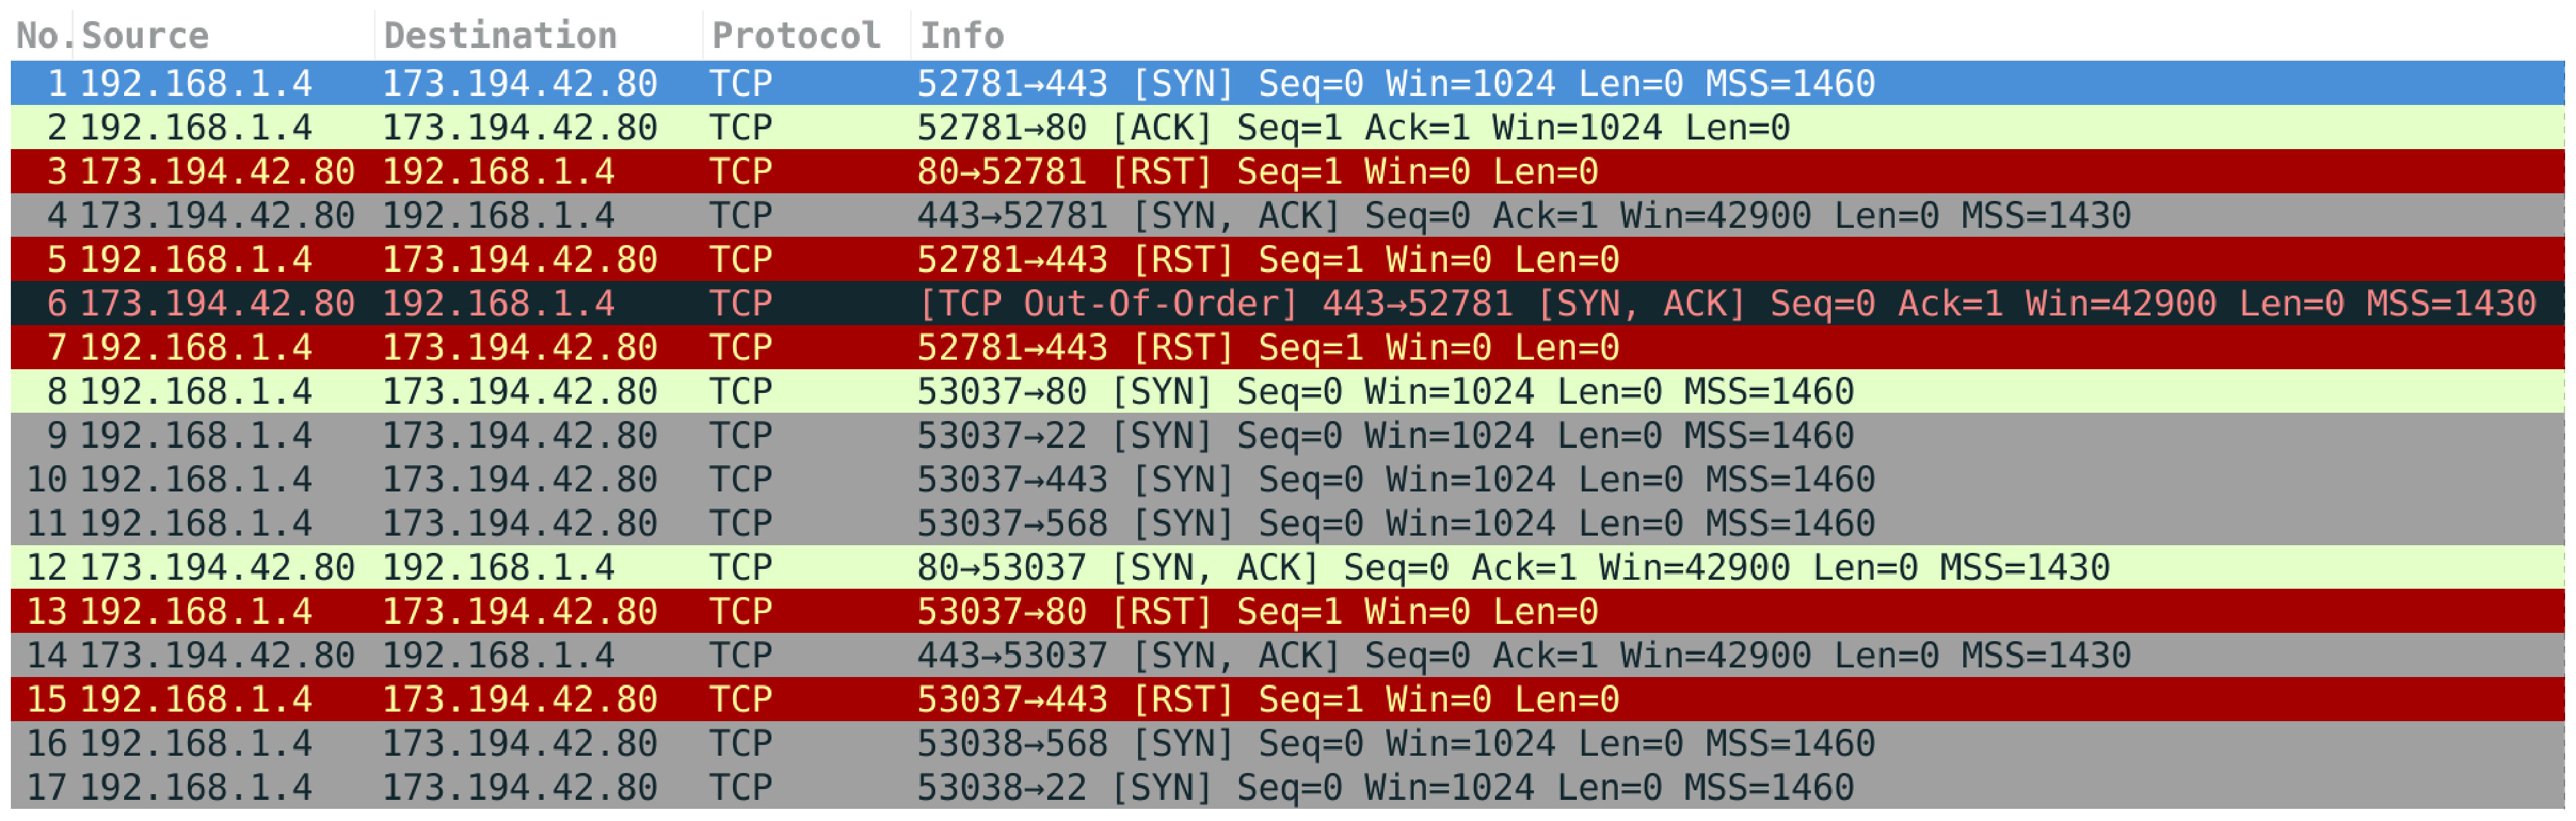
\includegraphics[width=0.9\textwidth]{figuras/captura_nmap.eps}
  \caption{Captura de pacotes Nmap}
  \label{fig:captura_nmap}
\end{figure}

Antes de analisar a figura de fato, vale ressaltar que apenas pacotes TCP estão
sendo filtrados. Isso foi feito para facilitar a análise dos segmentos sendo
usados, pois como uma url está sendo usada como parâmetro, uma consulta DNS
deverá ser feita para encontrar o endereço IP associado aquela url, mas os
pacotes trocados para realizar tal tarefa não interessam nesta prática.

Fazendo a análise propriamente dita, pode ser visto que a etapa de identificação de host pode ser vista nas linhas 1-7,
onde o Nmap tenta estabelecer conexões nas portas 80 e 443. Pode ser visto que o Nmap tenta mandar um TCP SYN para a porta
443 e um TCP ACK para a porta 80. Percebe-se que ambos os pacotes recebem uma resposta, mostrando que o host está ativo.

Nas linhas 8-11, pode ser visto o Nmap tentando enviar um pacote SYN para cada porta especificada. Nas linhas 12-13 percebe-se
que o Nmap recebeu um pacote TCP SYNACK da porta 80, ou seja, a porta é considerad aberta. Após isso, o Nmap fecha a conexão com
um TCP RST. Esse mesmo comportamento acontece nas linhas 14-15 para a porta 443. Para as outras portas, percebe-se que o Nmap começa a
retransmitir pacotes destinados aquela porta, identificando que talvez a porta esteja sendo filtrada.

A Figura \ref{fig:saida_nmap} mostra a saída obtida ao usar o nmap para executar o comando mostrado. Pode-se ver que a saída mostrada pelo Nmap corrabora
perfeitamente com a análise feita em cima da captura de pacotes.

\begin{figure}[h]
  \centering
  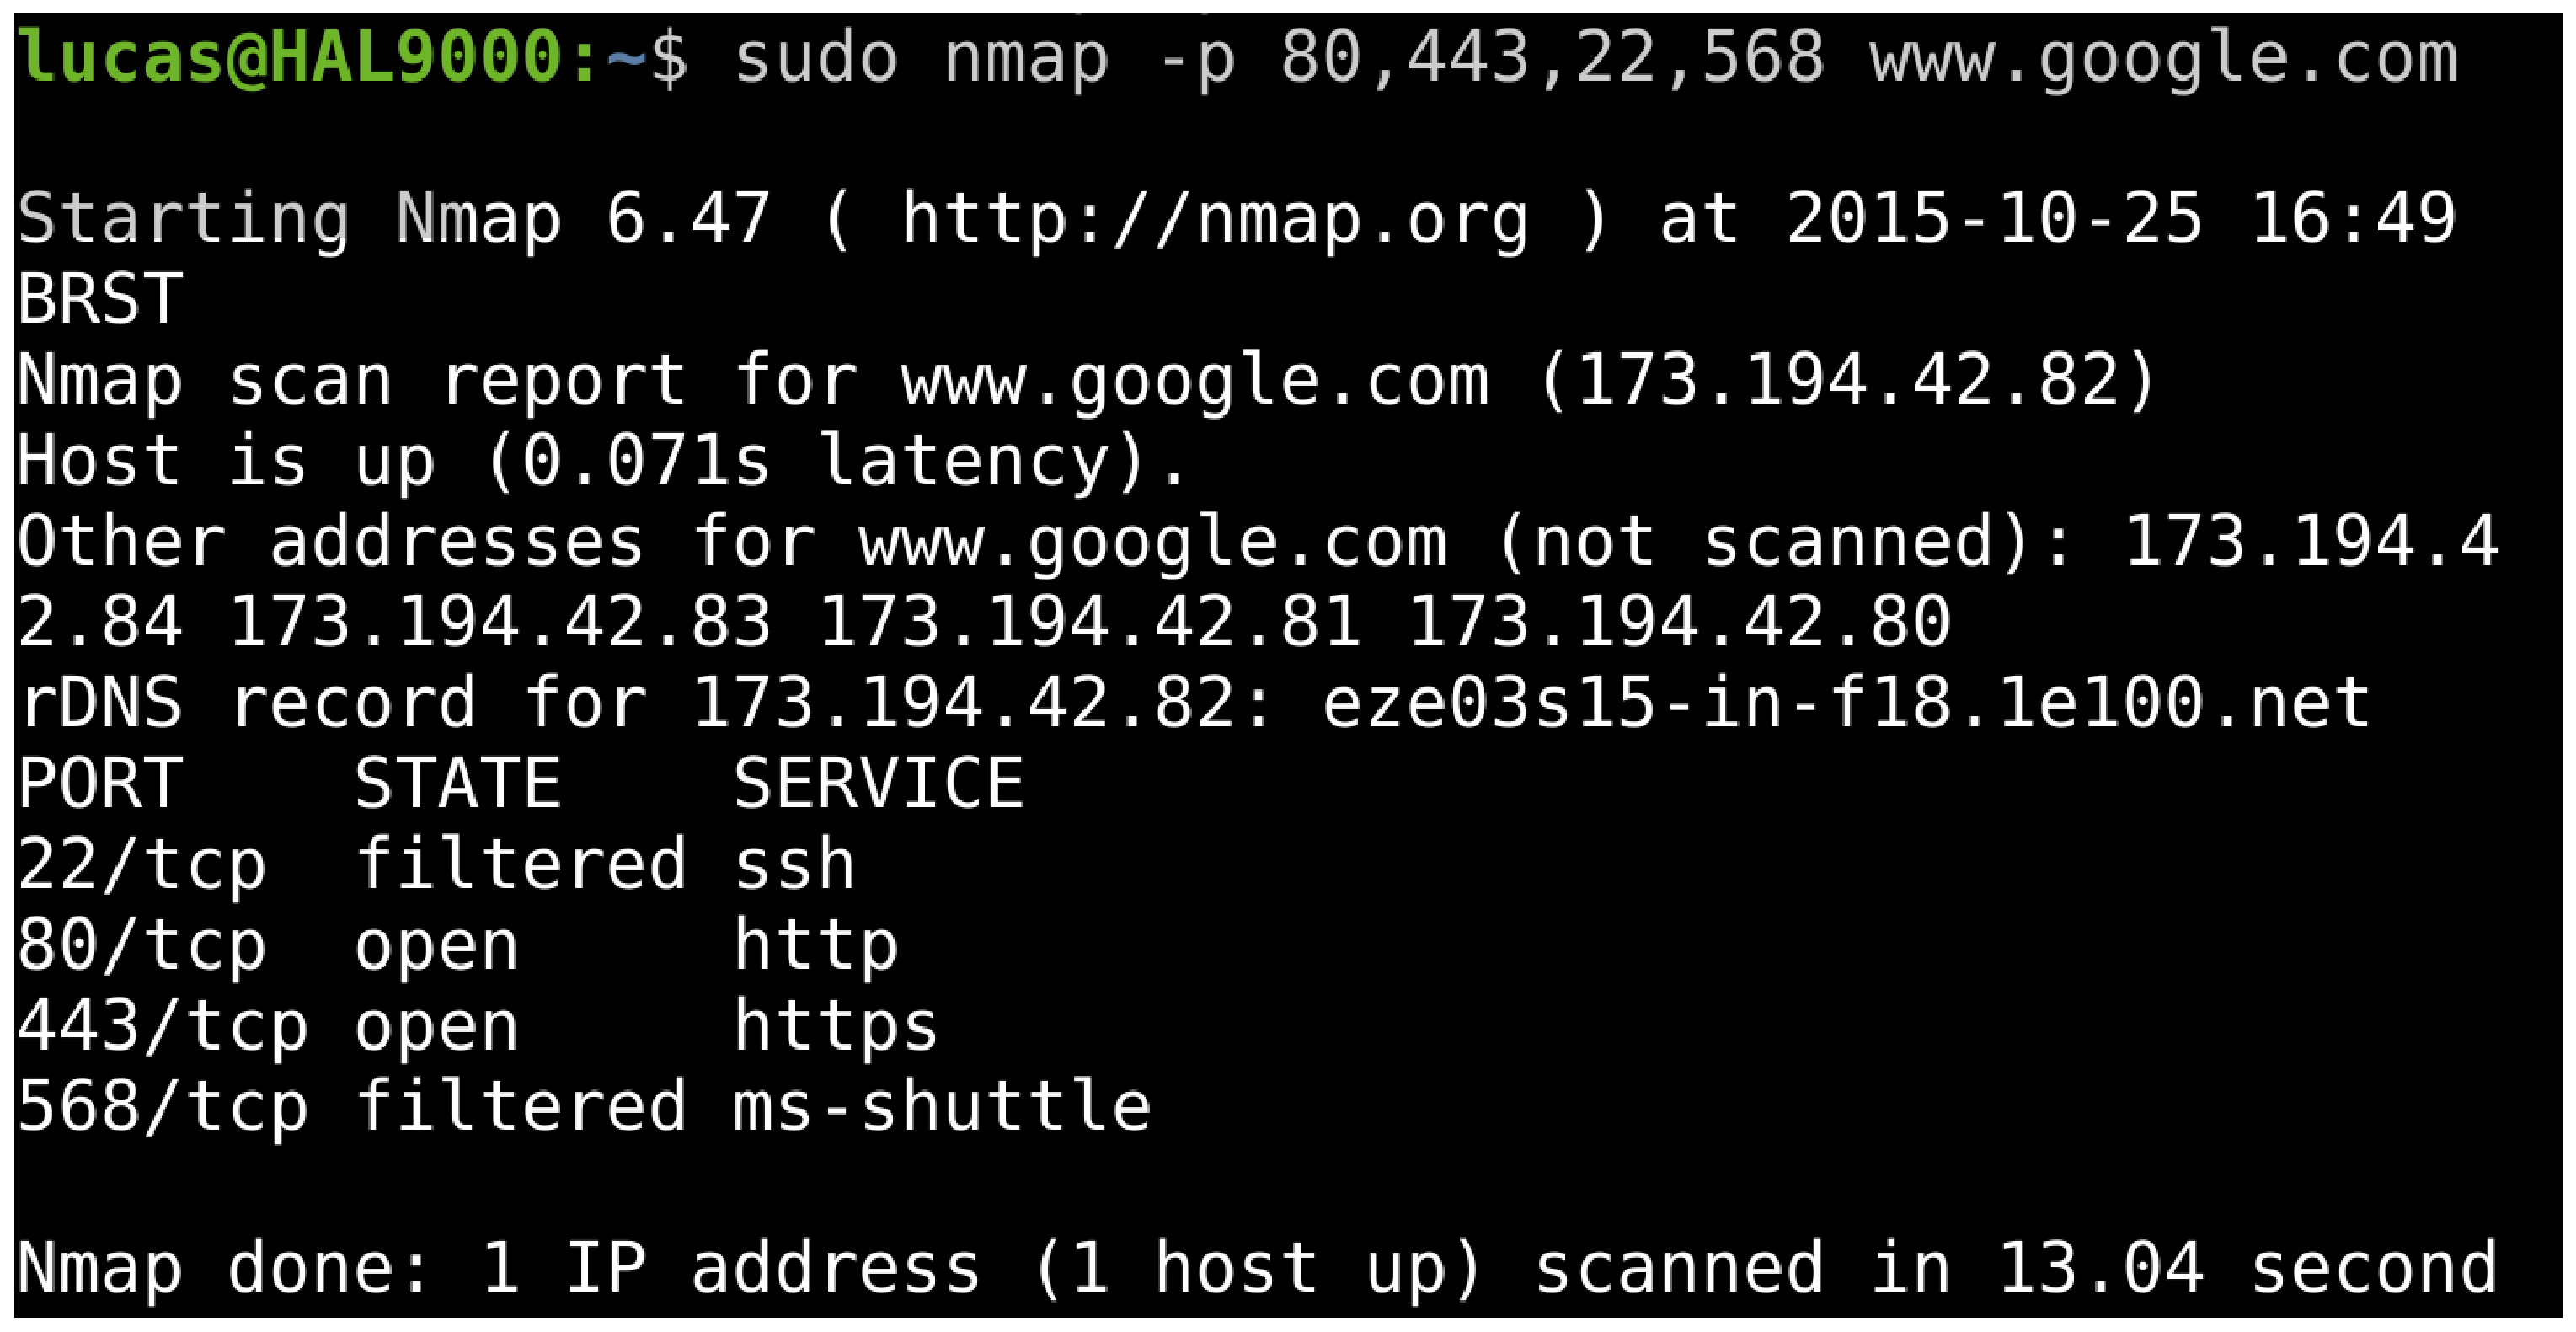
\includegraphics[width=0.9\textwidth]{figuras/saida_nmap.eps}
  \caption{Saída do comando Nmap}
  \label{fig:saida_nmap}
\end{figure}


Sendo assim, pode-se concluir que o Nmap usa o protocolo TCP da camada de transporte e o protocolo IP da camada de rede para executar suas funcionalidades
em uma chamada típica. Entretanto, vale ressaltar que o Nmap também pode ser usado de outras formas, permitindo scannear redes com protocolo UDP da camada de transporte
e até como o protocolo ICMP da camada de rede. Entretanto, para se usar tal funcionalidade é necessário com que o usuário passe algumas flags especiais na hora
de executar o comando, ou seja, não é o cenário típico de uso.


